% Options for packages loaded elsewhere
\PassOptionsToPackage{unicode}{hyperref}
\PassOptionsToPackage{hyphens}{url}
\PassOptionsToPackage{dvipsnames,svgnames,x11names}{xcolor}
%
\documentclass[
  letterpaper,
  DIV=11,
  numbers=noendperiod,
  oneside]{scrreprt}

\usepackage{amsmath,amssymb}
\usepackage{iftex}
\ifPDFTeX
  \usepackage[T1]{fontenc}
  \usepackage[utf8]{inputenc}
  \usepackage{textcomp} % provide euro and other symbols
\else % if luatex or xetex
  \usepackage{unicode-math}
  \defaultfontfeatures{Scale=MatchLowercase}
  \defaultfontfeatures[\rmfamily]{Ligatures=TeX,Scale=1}
\fi
\usepackage{lmodern}
\ifPDFTeX\else  
    % xetex/luatex font selection
\fi
% Use upquote if available, for straight quotes in verbatim environments
\IfFileExists{upquote.sty}{\usepackage{upquote}}{}
\IfFileExists{microtype.sty}{% use microtype if available
  \usepackage[]{microtype}
  \UseMicrotypeSet[protrusion]{basicmath} % disable protrusion for tt fonts
}{}
\makeatletter
\@ifundefined{KOMAClassName}{% if non-KOMA class
  \IfFileExists{parskip.sty}{%
    \usepackage{parskip}
  }{% else
    \setlength{\parindent}{0pt}
    \setlength{\parskip}{6pt plus 2pt minus 1pt}}
}{% if KOMA class
  \KOMAoptions{parskip=half}}
\makeatother
\usepackage{xcolor}
\usepackage[left=1in,marginparwidth=2.0666666666667in,textwidth=4.1333333333333in,marginparsep=0.3in]{geometry}
\setlength{\emergencystretch}{3em} % prevent overfull lines
\setcounter{secnumdepth}{5}
% Make \paragraph and \subparagraph free-standing
\ifx\paragraph\undefined\else
  \let\oldparagraph\paragraph
  \renewcommand{\paragraph}[1]{\oldparagraph{#1}\mbox{}}
\fi
\ifx\subparagraph\undefined\else
  \let\oldsubparagraph\subparagraph
  \renewcommand{\subparagraph}[1]{\oldsubparagraph{#1}\mbox{}}
\fi


\providecommand{\tightlist}{%
  \setlength{\itemsep}{0pt}\setlength{\parskip}{0pt}}\usepackage{longtable,booktabs,array}
\usepackage{calc} % for calculating minipage widths
% Correct order of tables after \paragraph or \subparagraph
\usepackage{etoolbox}
\makeatletter
\patchcmd\longtable{\par}{\if@noskipsec\mbox{}\fi\par}{}{}
\makeatother
% Allow footnotes in longtable head/foot
\IfFileExists{footnotehyper.sty}{\usepackage{footnotehyper}}{\usepackage{footnote}}
\makesavenoteenv{longtable}
\usepackage{graphicx}
\makeatletter
\def\maxwidth{\ifdim\Gin@nat@width>\linewidth\linewidth\else\Gin@nat@width\fi}
\def\maxheight{\ifdim\Gin@nat@height>\textheight\textheight\else\Gin@nat@height\fi}
\makeatother
% Scale images if necessary, so that they will not overflow the page
% margins by default, and it is still possible to overwrite the defaults
% using explicit options in \includegraphics[width, height, ...]{}
\setkeys{Gin}{width=\maxwidth,height=\maxheight,keepaspectratio}
% Set default figure placement to htbp
\makeatletter
\def\fps@figure{htbp}
\makeatother

\KOMAoption{captions}{tableheading}
\makeatletter
\@ifpackageloaded{tcolorbox}{}{\usepackage[skins,breakable]{tcolorbox}}
\@ifpackageloaded{fontawesome5}{}{\usepackage{fontawesome5}}
\definecolor{quarto-callout-color}{HTML}{909090}
\definecolor{quarto-callout-note-color}{HTML}{0758E5}
\definecolor{quarto-callout-important-color}{HTML}{CC1914}
\definecolor{quarto-callout-warning-color}{HTML}{EB9113}
\definecolor{quarto-callout-tip-color}{HTML}{00A047}
\definecolor{quarto-callout-caution-color}{HTML}{FC5300}
\definecolor{quarto-callout-color-frame}{HTML}{acacac}
\definecolor{quarto-callout-note-color-frame}{HTML}{4582ec}
\definecolor{quarto-callout-important-color-frame}{HTML}{d9534f}
\definecolor{quarto-callout-warning-color-frame}{HTML}{f0ad4e}
\definecolor{quarto-callout-tip-color-frame}{HTML}{02b875}
\definecolor{quarto-callout-caution-color-frame}{HTML}{fd7e14}
\makeatother
\makeatletter
\@ifpackageloaded{bookmark}{}{\usepackage{bookmark}}
\makeatother
\makeatletter
\@ifpackageloaded{caption}{}{\usepackage{caption}}
\AtBeginDocument{%
\ifdefined\contentsname
  \renewcommand*\contentsname{Table des matières}
\else
  \newcommand\contentsname{Table des matières}
\fi
\ifdefined\listfigurename
  \renewcommand*\listfigurename{Liste des Figures}
\else
  \newcommand\listfigurename{Liste des Figures}
\fi
\ifdefined\listtablename
  \renewcommand*\listtablename{Liste des Tables}
\else
  \newcommand\listtablename{Liste des Tables}
\fi
\ifdefined\figurename
  \renewcommand*\figurename{Figure}
\else
  \newcommand\figurename{Figure}
\fi
\ifdefined\tablename
  \renewcommand*\tablename{Table}
\else
  \newcommand\tablename{Table}
\fi
}
\@ifpackageloaded{float}{}{\usepackage{float}}
\floatstyle{ruled}
\@ifundefined{c@chapter}{\newfloat{codelisting}{h}{lop}}{\newfloat{codelisting}{h}{lop}[chapter]}
\floatname{codelisting}{Listing}
\newcommand*\listoflistings{\listof{codelisting}{Liste des Listings}}
\makeatother
\makeatletter
\makeatother
\makeatletter
\@ifpackageloaded{caption}{}{\usepackage{caption}}
\@ifpackageloaded{subcaption}{}{\usepackage{subcaption}}
\makeatother
\makeatletter
\@ifpackageloaded{sidenotes}{}{\usepackage{sidenotes}}
\@ifpackageloaded{marginnote}{}{\usepackage{marginnote}}
\makeatother
\ifLuaTeX
\usepackage[bidi=basic]{babel}
\else
\usepackage[bidi=default]{babel}
\fi
\babelprovide[main,import]{french}
% get rid of language-specific shorthands (see #6817):
\let\LanguageShortHands\languageshorthands
\def\languageshorthands#1{}
\ifLuaTeX
  \usepackage{selnolig}  % disable illegal ligatures
\fi
\usepackage{bookmark}

\IfFileExists{xurl.sty}{\usepackage{xurl}}{} % add URL line breaks if available
\urlstyle{same} % disable monospaced font for URLs
% Make links footnotes instead of hotlinks:
\DeclareRobustCommand{\href}[2]{#2\sidenote{\footnotesize \url{#1}}}
\hypersetup{
  pdftitle={Atelier Tropy},
  pdfauthor={Mélanie Le Couédic; Julien Rabaud},
  pdflang={fr},
  colorlinks=true,
  linkcolor={blue},
  filecolor={Maroon},
  citecolor={Blue},
  urlcolor={Blue},
  pdfcreator={LaTeX via pandoc}}

\title{Atelier Tropy}
\usepackage{etoolbox}
\makeatletter
\providecommand{\subtitle}[1]{% add subtitle to \maketitle
  \apptocmd{\@title}{\par {\large #1 \par}}{}{}
}
\makeatother
\subtitle{dans le cadre des jeudis d'ITEM}
\author{Mélanie Le Couédic \and Julien Rabaud}
\date{2024-05-16}

\begin{document}
\maketitle

\renewcommand*\contentsname{Table des matières}
{
\hypersetup{linkcolor=}
\setcounter{tocdepth}{2}
\tableofcontents
}
\bookmarksetup{startatroot}

\chapter*{Accueil}\label{accueil}
\addcontentsline{toc}{chapter}{Accueil}

\markboth{Accueil}{Accueil}

\begin{tcolorbox}[enhanced jigsaw, arc=.35mm, colback=white, rightrule=.15mm, bottomrule=.15mm, leftrule=.75mm, colframe=quarto-callout-tip-color-frame, opacityback=0, breakable, left=2mm, toprule=.15mm]

\begin{figure}[H]

\begin{minipage}{0.33\linewidth}

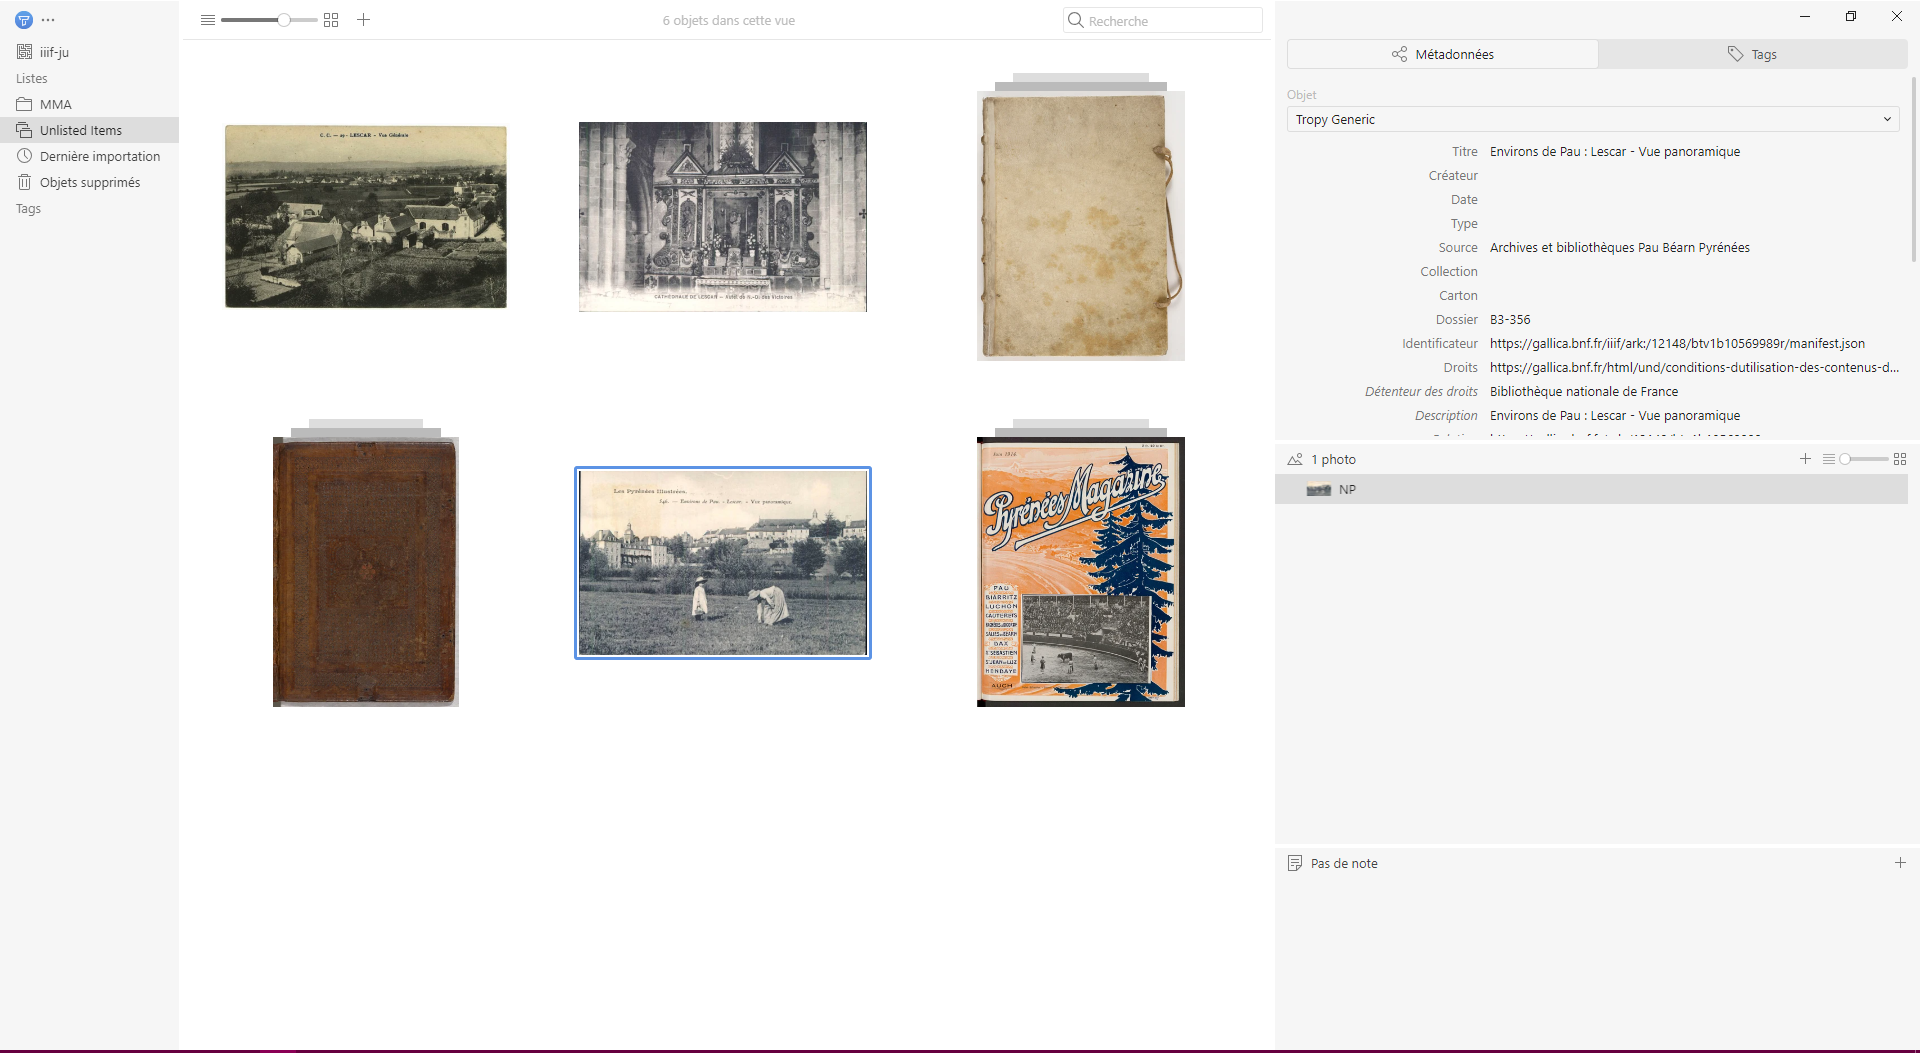
\includegraphics{img/tropy_items-gallerie.png}

\subcaption{\label{}Tropy - Vue items en gallerie}
\end{minipage}%
%
\begin{minipage}{0.33\linewidth}

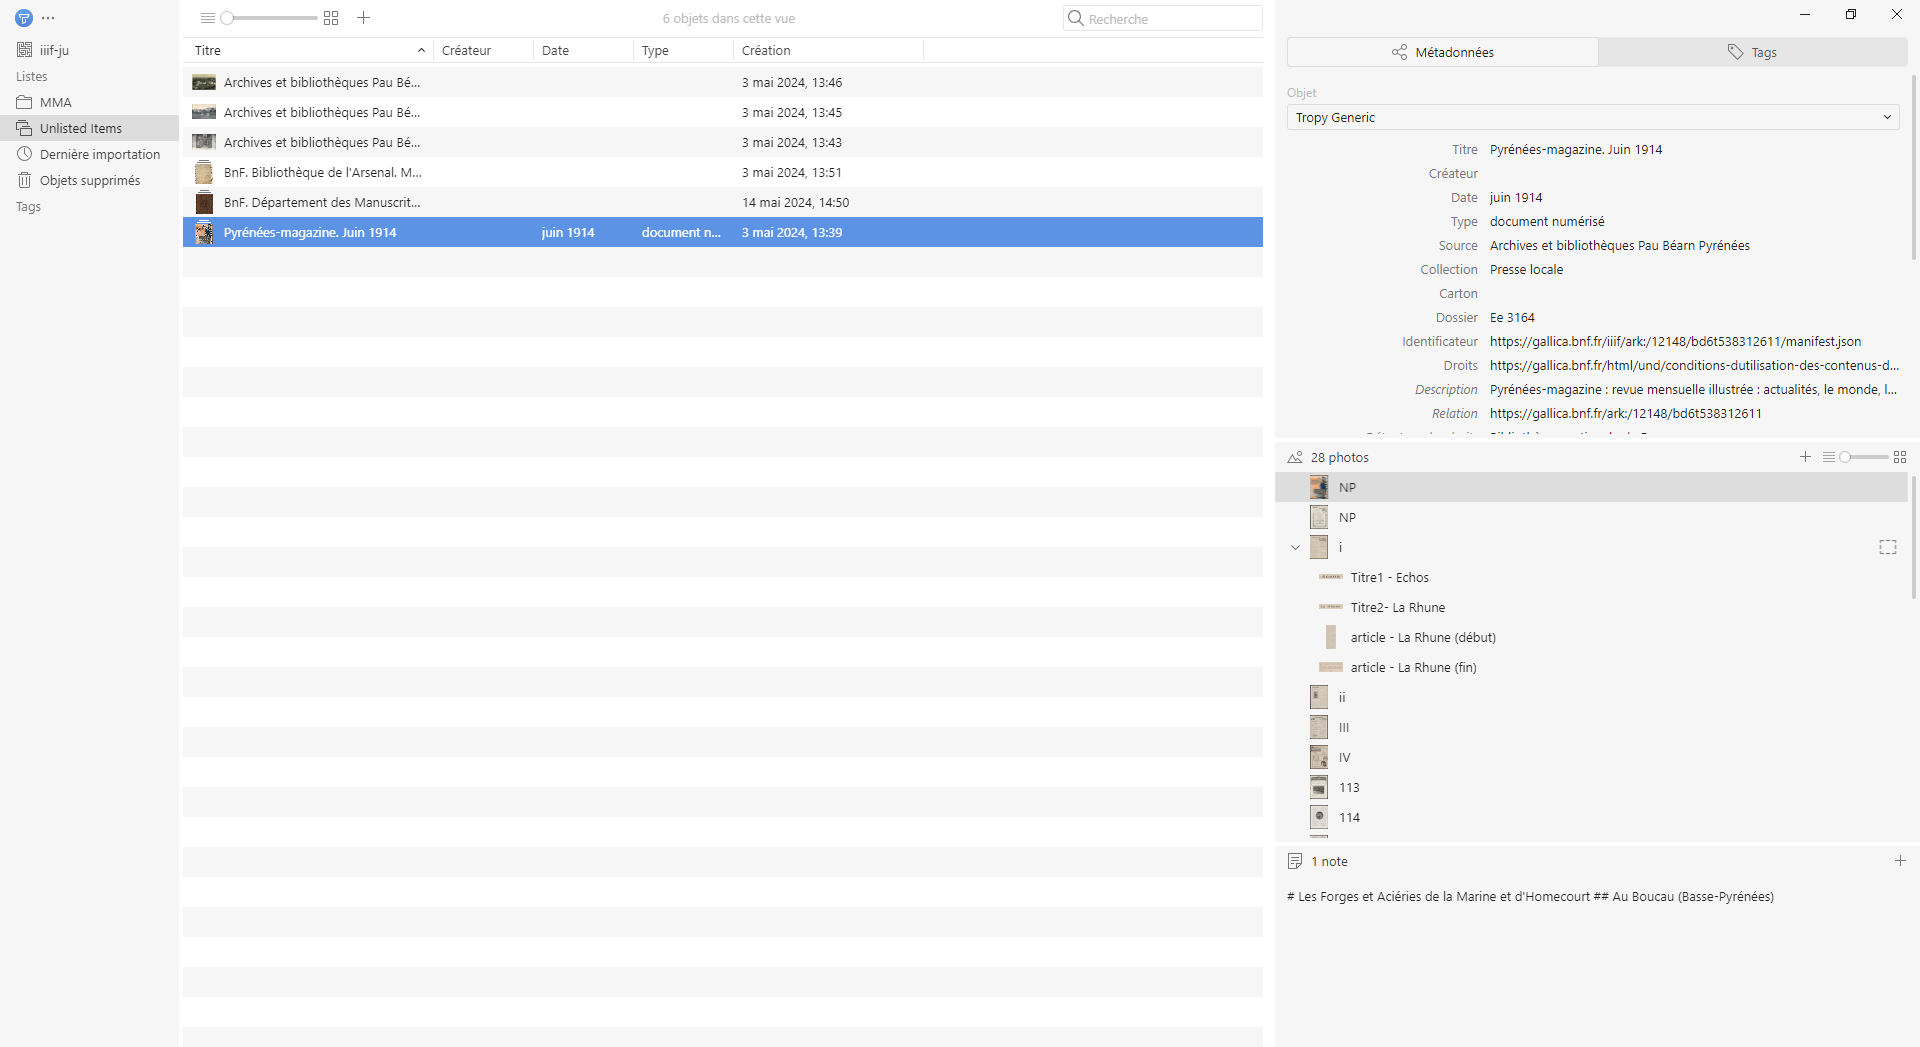
\includegraphics{img/tropy_items-liste.png}

\subcaption{\label{}Tropy - Vue items en liste}
\end{minipage}%
%
\begin{minipage}{0.33\linewidth}


\includegraphics{img/tropy_vue-photo.png}

\subcaption{\label{}Tropy - Photo et sélections}
\end{minipage}%

\end{figure}%

\end{tcolorbox}

\href{https://tropy.org}{\textbf{Tropy}} est un logiciel de gestion
d'images pour la Recherche

\begin{itemize}
\tightlist
\item
  scans de documents anciens
\item
  photographies d'archives
\item
  photographies de terrain
\item
  \ldots{}
\end{itemize}

Fait par des chercheurs pour des chercheurs par
\href{https://digitalscholar.org/}{Digital Scholar} (comme
\href{https://www.zotero.org/}{Zotero} et
\href{https://omeka.org/}{Omeka})

\begin{tcolorbox}[enhanced jigsaw, arc=.35mm, colback=white, rightrule=.15mm, bottomrule=.15mm, leftrule=.75mm, colframe=quarto-callout-note-color-frame, opacityback=0, breakable, left=2mm, toprule=.15mm]

\begin{figure}[H]

\begin{minipage}{0.50\linewidth}


\includegraphics[width=\textwidth,height=1.92708in]{img/jeudi-ditem-1-1-1038x576-1.jpg}

\subcaption{\label{}\href{https://item.univ-pau.fr/fr/activites-scientifiques/jeudis-d-item.html}{Les
jeudis d'ITEM}}
\end{minipage}%
%
\begin{minipage}{0.50\linewidth}


\includegraphics[width=\textwidth,height=1.92708in]{img/tropy-app-icon-1024x1024.png}

\subcaption{\label{}\href{https://tropy.org}{Tropy}}
\end{minipage}%

\end{figure}%

\end{tcolorbox}

\part{Ressources sur Tropy}

\phantomsection\label{ressources}

\chapter{Tropy, canaux officels}\label{tropy-canaux-officels}

\begin{itemize}
\tightlist
\item
  \href{https://docs.tropy.org/}{Documentation}
\item
  \href{https://forums.tropy.org/}{Support} (forum)
\item
  \href{https://vimeo.com/user73164761}{Vimeo}
\item
  \href{https://www.youtube.com/watch?v=jWjP90EWHkQ&feature=youtu.be}{Youtube}
\item
  \href{https://twitter.com/tropy}{Twitter}
\item
  \href{https://github.com/tropy}{GitHub} (code source, templates\ldots)
\end{itemize}

\chapter{Extensions pour Tropy}\label{extensions-pour-tropy}

\begin{figure}[H]

{\centering 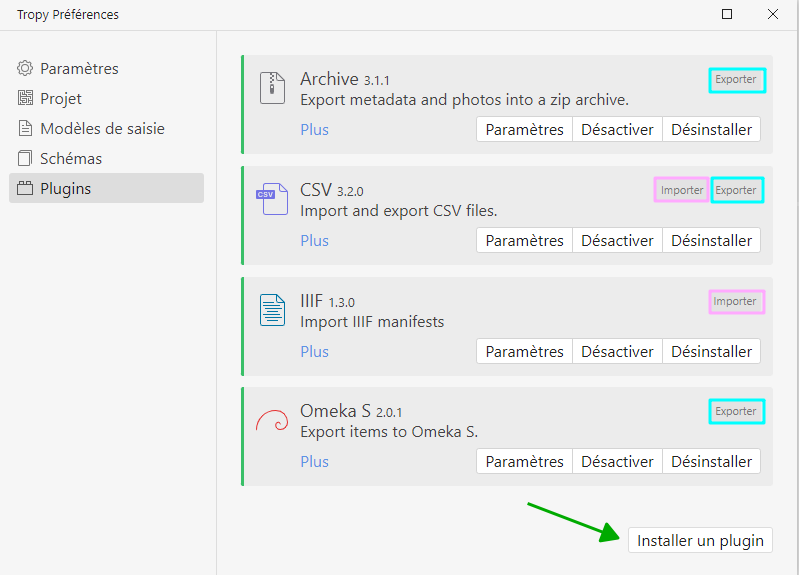
\includegraphics[width=0.7\textwidth,height=\textheight]{img/tropy-plugins.png}

}

\caption{Menu: Préférences\ldots{} - Plugins}

\end{figure}%

\begin{longtable}[]{@{}
  >{\raggedright\arraybackslash}p{(\columnwidth - 2\tabcolsep) * \real{0.3000}}
  >{\raggedright\arraybackslash}p{(\columnwidth - 2\tabcolsep) * \real{0.7000}}@{}}
\caption{Table des extensions}\tabularnewline
\toprule\noalign{}
\begin{minipage}[b]{\linewidth}\raggedright
Nom (et lien)
\end{minipage} & \begin{minipage}[b]{\linewidth}\raggedright
Description
\end{minipage} \\
\midrule\noalign{}
\endfirsthead
\toprule\noalign{}
\begin{minipage}[b]{\linewidth}\raggedright
Nom (et lien)
\end{minipage} & \begin{minipage}[b]{\linewidth}\raggedright
Description
\end{minipage} \\
\midrule\noalign{}
\endhead
\bottomrule\noalign{}
\endlastfoot
\href{https://github.com/tropy/tropy-plugin-csl}{tropy-plugin-csl} &
Tropy plugin to export \emph{your} items to Zotero as CSL/JSON \\
\href{https://github.com/tropy/tropy-plugin-omeka}{tropy-plugin-omeka} &
This plugin can export selected items into an
\href{https://omeka.org/s/}{Omeka S} instance. \\
\href{https://github.com/tropy/tropy-plugin-archive}{tropy-plugin-archive}
& Tropy plugin for exporting items into a single zip archive. This
includes all the metadata, as well as the photo files. \\
\href{https://github.com/tropy/tropy-plugin-csv}{tropy-plugin-csv} &
Tropy plugin to import items from a CSV file, and export your items to
CSV. \\
\href{https://github.com/tropy/tropy-plugin-iiif}{tropy-plugin-iiif} &
Download a IIIF manifest and select~\emph{File \textgreater{} Import
\textgreater{} tropy-plugin-iiif}~to start the import. The plugin tries
to map the manifest's metadata to standard metadata properties. \\
\end{longtable}

\chapter{Tutoriels sur Tropy}\label{tutoriels-sur-tropy}

\begin{longtable}[]{@{}
  >{\raggedright\arraybackslash}p{(\columnwidth - 2\tabcolsep) * \real{0.5000}}
  >{\raggedright\arraybackslash}p{(\columnwidth - 2\tabcolsep) * \real{0.5000}}@{}}
\caption{Table des Tutoriels Tropy}\tabularnewline
\toprule\noalign{}
\begin{minipage}[b]{\linewidth}\raggedright
Auteur
\end{minipage} & \begin{minipage}[b]{\linewidth}\raggedright
lien
\end{minipage} \\
\midrule\noalign{}
\endfirsthead
\toprule\noalign{}
\begin{minipage}[b]{\linewidth}\raggedright
Auteur
\end{minipage} & \begin{minipage}[b]{\linewidth}\raggedright
lien
\end{minipage} \\
\midrule\noalign{}
\endhead
\bottomrule\noalign{}
\endlastfoot
Benjamin Lailler & \href{https://zenodo.org/record/2583661}{Tutoriel
Tropy} \\
Stretching numérique 2023 &
\href{https://zenodo.org/records/7762441}{Gérer ses photos d'archives
avec Tropy} \\
York Library &
\href{https://yorkspace.library.yorku.ca/xmlui/bitstream/handle/10315/36607/Handout-Tropy\%20and\%20Archival\%20Fieldwork.pdf?sequence=3&isAllowed=y}{Handout
- Tropy and Archival Fieldwork (2 p.)} \\
George Mason University Library &
\href{https://infoguides.gmu.edu/tropy/introduction}{Infoguide Tropy} \\
Schlesinger Library on the History of Women in America - Harvard
University &
\href{https://guides.library.harvard.edu/c.php?g=833532&p=5990005}{Tropy
Guide} \\
BULAC 2022-04 &
\href{https://www.bulac.fr/document/support-de-formation-tropy-2022-04}{Support
de formation - Tropy} \\
Université de Lille - \emph{Pole-Num-Scrums-Skills} &
\href{https://wikis.univ-lille.fr/proj-polnum/accueil/manuels/guide-d-utilisation-de-tropy}{Tropy
\textbar{} gestion d'images} \\
Rennes 2 & \href{https://tutos.bu.univ-rennes2.fr/c.php?g=702342}{Gérer
ses photos de recherche avec Tropy} \\
\end{longtable}

\chapter{Vidéos sur Tropy}\label{viduxe9os-sur-tropy}

\begin{itemize}
\item
  Le 16 juin 2020, L'équipe de Tropy (Abby Mullen) a tenu un webinaire
  de type \emph{Tropy 101}
  {[}\href{https://www.youtube.com/watch?v=Hk5APGD6200}{Youtube -
  1h05}{]}

  \url{https://www.youtube.com/embed/jWjP90EWHkQ}
\item
  Tropy chanel : \emph{Metadata Templates in Tropy}
  {[}\href{https://www.youtube.com/watch?v=Hk5APGD6200}{Youtube - 10
  mn}{]}

  \url{https://www.youtube.com/embed/Hk5APGD6200}
\end{itemize}

\begin{itemize}
\item
  \href{https://eveille.hypotheses.org/}{Projet EVEille} : Séance
  d'initiation à Tropy, animée par~Benoît~Roux, juin 2021
  {[}\href{https://e-diffusion.uha.fr/video/4023-initiation-a-tropy-avril-2021/}{e-diffusion
  UHA - 1h28}{]}

  \url{https://e-diffusion.uha.fr/video/4023-initiation-a-tropy-avril-2021}
\item
  Geneatech : \emph{Utiliser Tropy pour la gestion de ses photos
  d'archive}
  {[}\href{https://www.youtube.com/watch?v=AiPqbdwP67E}{Youtube - 17
  mn}{]}

  \url{https://www.youtube.com/embed/AiPqbdwP67E}
\end{itemize}

\chapter{Billets de blog}\label{billets-de-blog}

\begin{itemize}
\tightlist
\item
  \href{http://www.boiteaoutils.info/2017/10/gerer-ses-photos-darchives-avec-tropy/}{Gérer
  ses photos d'archives avec Tropy} - Franziska Heimburger - \emph{La
  boîte à outils des historien·ne·s} (2017)
\item
  \href{https://www.macg.co/logiciels/2017/10/tropy-un-gestionnaire-de-photos-darchives-pour-les-chercheurs-100197}{Tropy,
  un gestionnaire de photos d'archives pour les~chercheurs} - Florian
  Innocente, \emph{MacGeneration} (2017)
\item
  \href{https://www.e-mourlon-druol.com/six-months-of-using-tropy/}{Six
  months of using Tropy} - Emmanuel Mourlon-Druol (2019)
\item
  \href{https://bulac.hypotheses.org/33406}{Tropy : un logiciel pour
  organiser des corpus iconographiques} - BULAC (2021)
\item
  \href{https://tropy.org/blog/new-project-types-in-tropy-1-13}{New
  Project Types in Tropy 1.13} - Tropy Blog (2023-03-31)
\end{itemize}

\part{Prise en main}

\phantomsection\label{main}

\chapter{Créer un projet}\label{cruxe9er-un-projet}

\begin{figure}[H]

{\centering 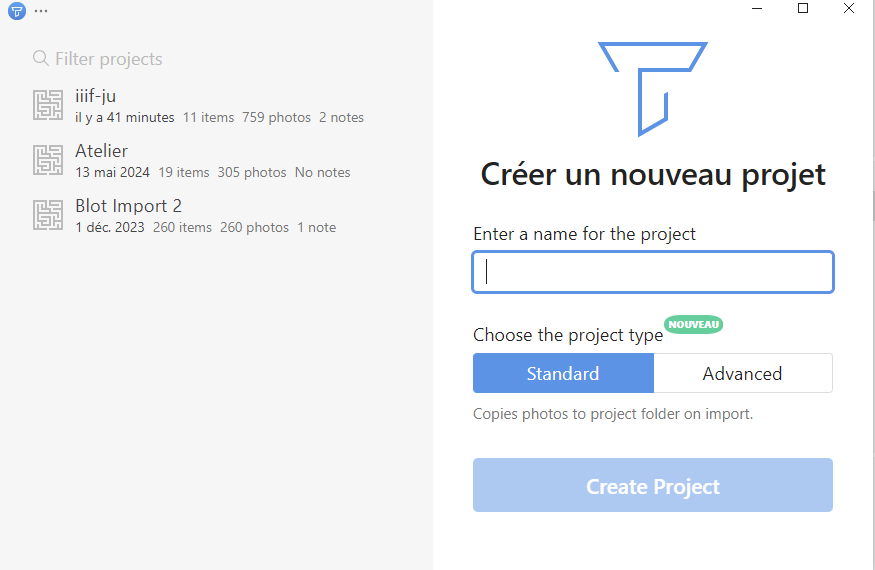
\includegraphics{img/tropy-projet.png}

}

\caption{Menu: Fichier \textgreater{} Nouveau \textgreater{} Projet
(Ctrl+Maj+P)}

\end{figure}%

\begin{itemize}
\tightlist
\item
  Lui donner un nom
\item
  Choisir le type (voir
  \href{https://tropy.org/blog/new-project-types-in-tropy-1-13}{New
  Project Types in Tropy 1.13})

  \begin{itemize}
  \tightlist
  \item
    \emph{Standard} : Copie les photos dans le dossier du projet à
    l'import
  \item
    \emph{Advanced} : Lien vers les photos sur votre disque
    (/!\textbackslash)
  \end{itemize}
\end{itemize}

\chapter{Les modèles de documents}\label{les-moduxe8les-de-documents}

\section{Dans la documentation
officielle}\label{dans-la-documentation-officielle}

\begin{itemize}
\tightlist
\item
  \href{https://docs.tropy.org/before-you-begin/metadata}{What is
  metadata and how do I use it?}
\item
  \href{https://docs.tropy.org/in-the-template-editor/using-templates}{Getting
  started with templates}
\end{itemize}

\subsection{Exemple du Projet Blot}\label{exemple-du-projet-blot}

\begin{itemize}
\tightlist
\item
  Template \texttt{Blot\ photos\ v2} :
  \href{BlotPhotosV2.ttp}{Télécharger}

  \begin{itemize}
  \tightlist
  \item
    \href{https://git.univ-pau.fr/gaelannuzelt/projet-blot/-/wikis/Templates-Tropy}{Description
    dans le wiki du projet}
  \end{itemize}
\end{itemize}

\chapter{Importer des photos}\label{importer-des-photos}

Formats supportés :

\begin{itemize}
\tightlist
\item
  JPG/JPEG
\item
  PNG
\item
  SVG
\item
  TIFF
\item
  GIF
\item
  PDF
\item
  JP2000
\item
  WEBP
\item
  HEIC
\item
  AVIF
\end{itemize}

\section{Menu: Fichier \textgreater{} Importer \textgreater{} Photos
\textbar{} Dossier}\label{menu-fichier-importer-photos-dossier}

\begin{itemize}
\tightlist
\item
  Penser à définir un profil d'import par défaut avant.
\end{itemize}

\section{Glisser-déposer}\label{glisser-duxe9poser}

\begin{itemize}
\tightlist
\item
  Même recommandation
\end{itemize}

\section{Surveillance d'un dossier}\label{surveillance-dun-dossier}

\begin{itemize}
\tightlist
\item
  Menu: Edition \textgreater{} Préférences\ldots{} \textbar{} onglet
  \emph{Projet} -\textgreater{} Watch folder
\end{itemize}

\section{Plugins}\label{plugins}

\subsection{CSV}\label{csv}

\begin{enumerate}
\def\labelenumi{\arabic{enumi}.}
\tightlist
\item
  Installer le \href{https://github.com/tropy/tropy-plugin-csv}{plugin
  CSV}
\item
  \begin{enumerate}
  \def\labelenumii{\arabic{enumii}.}
  \tightlist
  \item
    Menu: Edition \textgreater{} Préférences\ldots{} \textbar{} onglet
    \emph{Plugins} -\textgreater{} Définir un profil d'import CSV
  \end{enumerate}
\end{enumerate}

\subsection{IIIF}\label{iiif}

\begin{enumerate}
\def\labelenumi{\arabic{enumi}.}
\tightlist
\item
  Installer le \href{https://github.com/tropy/tropy-plugin-iiif}{plugin
  IIIF}
\item
  Menu: Edition \textgreater{} Préférences\ldots{} \textbar{} onglet
  \emph{Plugins} -\textgreater{} Définir un profil d'import (template)
  IIIF dans les \textbf{paramètres} du plugin.
\item
  Télécharger un \emph{manifeste IIIF} (souvent un fichier
  \texttt{manifest.json}) sur son ordinateur depuis un catalogue IIIF
  (Gallica, Biblissima, Europeana..)
\item
  Dans Tropy, Menu: Fichier \textgreater{} Importer \textgreater{}
  Profil IIIF : chemin du fichier \texttt{manifest.json}
\end{enumerate}

\chapter{Exporter (projet, photos,
données)}\label{exporter-projet-photos-donnuxe9es}

\section{Préférences \textgreater{}
Export}\label{pruxe9fuxe9rences-export}

\section{Menu Exporter}\label{menu-exporter}

\begin{itemize}
\tightlist
\item
  JSON-LD : LD pour \emph{Linked Data}
\item
  PDF
\item
  Plugins
\end{itemize}

\section{Plugins}\label{plugins-1}

\begin{itemize}
\tightlist
\item
  Archive : Photos et métadonnées dans un \texttt{.zip}
\item
  CSV
\item
  Omeka S
\end{itemize}

\bookmarksetup{startatroot}

\chapter*{Principes FAIR}\label{principes-fair}
\addcontentsline{toc}{chapter}{Principes FAIR}

\markboth{Principes FAIR}{Principes FAIR}

\begin{itemize}
\tightlist
\item
  Inspirés par le \emph{5-Star Open Data} proné par Tim-Berners Lee, mis
  en forme par Michael Hausenblas sur ce site :
  \url{http://5stardata.info/fr/} {[}22 janvier 2012{]}.
\end{itemize}

\begin{tcolorbox}[enhanced jigsaw, bottomtitle=1mm, coltitle=black, opacitybacktitle=0.6, colbacktitle=quarto-callout-important-color!10!white, colframe=quarto-callout-important-color-frame, left=2mm, arc=.35mm, colback=white, rightrule=.15mm, bottomrule=.15mm, leftrule=.75mm, toptitle=1mm, title=\textcolor{quarto-callout-important-color}{\faExclamation}\hspace{0.5em}{Les étapes \emph{5-Star OpenData}}, opacityback=0, breakable, titlerule=0mm, toprule=.15mm]

\begin{longtable}[]{@{}
  >{\raggedright\arraybackslash}p{(\columnwidth - 2\tabcolsep) * \real{0.2000}}
  >{\raggedright\arraybackslash}p{(\columnwidth - 2\tabcolsep) * \real{0.8000}}@{}}
\caption{Illustration des étapes \emph{5-Star OpenData}}\tabularnewline
\toprule\noalign{}
\begin{minipage}[b]{\linewidth}\raggedright
étoiles
\end{minipage} & \begin{minipage}[b]{\linewidth}\raggedright
étape
\end{minipage} \\
\midrule\noalign{}
\endfirsthead
\toprule\noalign{}
\begin{minipage}[b]{\linewidth}\raggedright
étoiles
\end{minipage} & \begin{minipage}[b]{\linewidth}\raggedright
étape
\end{minipage} \\
\midrule\noalign{}
\endhead
\bottomrule\noalign{}
\endlastfoot
★ & Publiez vos données sur le Web (peu importe leur format) avec une
licence ouverte \\
★★ & Publiez-les en tant que données structurées (par exemple, un
document Excel au lieu d'une image scannée d'un tableau) \\
★★★ & Publiez-les dans un format ouvert et non-propriétaire (par
exemple, un CSV plutôt qu'un Excel) \\
★★★★ & Utilisez des URI pour désigner des choses dans vos données, afin
que les gens puissent faire des références à celles-ci \\
★★★★★ & liez vos données à d'autres données pour y ajouter du
contexte \\
\end{longtable}

\end{tcolorbox}

\begin{itemize}
\tightlist
\item
  Décrits \href{https://www.go-fair.org/fair-principles/}{ici},
  d'après\emph{The FAIR Guiding Principles for Scientific Data
  Management and Stewardship}.
  \href{https://doi.org/10.1038/sdata.2016.18}{DOI}
\end{itemize}

\begin{quote}
\emph{The principles refer to three types of entities: \textbf{data} (or
any digital object), \textbf{metadata} (information about that digital
object), and \textbf{infrastructure}. For instance, principle
\href{https://www.go-fair.org/fair-principles/f4-metadata-registered-indexed-searchable-resource/}{F4}
defines that both metadata and data are registered or indexed in a
searchable resource (the infrastructure component).}
\end{quote}

\section{Findable}

\emph{The first step in (re)using data is to find them. Metadata and
data should be easy to find for both humans and computers.
Machine-readable metadata are essential for automatic discovery of
datasets and services, so this is an essential component of the
\href{https://www.go-fair.org/fair-principles/fairification-process/}{FAIRification
process}}.

\begin{itemize}
\tightlist
\item
  \href{https://www.go-fair.org/fair-principles/fair-data-principles-explained/f1-meta-data-assigned-globally-unique-persistent-identifiers/}{\textbf{F1}.
  (Meta)data are assigned a globally unique and \textbf{persistent
  identifier}}
\item
  \href{https://www.go-fair.org/fair-principles/fair-data-principles-explained/f2-data-described-rich-metadata/}{\textbf{F2}.
  Data are described with \textbf{rich metadata} (defined by R1 below)}
\item
  \href{https://www.go-fair.org/fair-principles/f3-metadata-clearly-explicitly-include-identifier-data-describe/}{\textbf{F3}.
  Metadata clearly and explicitly include the identifier of the data
  they describe}
\item
  \href{https://www.go-fair.org/fair-principles/f4-metadata-registered-indexed-searchable-resource/}{\textbf{F4}.
  (Meta)data are registered or indexed in a searchable resource}
\end{itemize}

\section{Accessible}

\emph{Once the user finds the required data, she/he/they need to know
how can they be accessed, possibly including authentication and
authorisation.}

\begin{itemize}
\tightlist
\item
  \href{https://www.go-fair.org/fair-principles/542-2/}{\textbf{A1}.
  (Meta)data are retrievable by their identifier using a standardised
  communications protocol}

  \begin{itemize}
  \tightlist
  \item
    \href{https://www.go-fair.org/fair-principles/a1-1-protocol-open-free-universally-implementable/}{\textbf{A1.1}
    The protocol is open, free, and universally implementable}
  \item
    \href{https://www.go-fair.org/fair-principles/a1-2-protocol-allows-authentication-authorisation-required/}{\textbf{A1.2}
    The protocol allows for an authentication and authorisation
    procedure, where necessary}
  \end{itemize}
\item
  \href{https://www.go-fair.org/fair-principles/a2-metadata-accessible-even-data-no-longer-available/}{\textbf{A2}.
  Metadata are accessible, even when the data are no longer available}
\end{itemize}

\section{Interoperable}

\emph{The data usually need to be integrated with other data. In
addition, the data need to interoperate with applications or workflows
for analysis, storage, and processing.}

\begin{itemize}
\item
  \href{https://www.go-fair.org/fair-principles/i1-metadata-use-formal-accessible-shared-broadly-applicable-language-knowledge-representation/}{\textbf{I1}.
  (Meta)data use a formal, accessible, shared, and broadly applicable
  language for knowledge representation.}
\item
  \href{https://www.go-fair.org/fair-principles/i2-metadata-use-vocabularies-follow-fair-principles/}{\textbf{I2}.
  (Meta)data use vocabularies that follow FAIR principles}
\item
  \href{https://www.go-fair.org/fair-principles/i3-metadata-include-qualified-references-metadata/}{\textbf{I3}.
  (Meta)data include qualified references to other (meta)data}
\end{itemize}

\section{Reusable}

\emph{The ultimate goal of FAIR is to optimise the reuse of data. To
achieve this, metadata and data should be well-described so that they
can be replicated and/or combined in different settings.}

\begin{itemize}
\item
  \href{https://www.go-fair.org/fair-principles/r1-metadata-richly-described-plurality-accurate-relevant-attributes/}{\textbf{R1}.
  (Meta)data are richly described with a plurality of accurate and
  relevant attributes}

  \begin{itemize}
  \item
    \href{https://www.go-fair.org/fair-principles/r1-1-metadata-released-clear-accessible-data-usage-license/}{\textbf{R1.1}.
    (Meta)data are released with a clear and accessible data usage
    license}
  \item
    \href{https://www.go-fair.org/fair-principles/r1-2-metadata-associated-detailed-provenance/}{\textbf{R1.2}.
    (Meta)data are associated with detailed provenance}
  \item
    \href{https://www.go-fair.org/fair-principles/r1-3-metadata-meet-domain-relevant-community-standards/}{\textbf{R1.3}.
    (Meta)data meet domain-relevant community standards}
  \end{itemize}
\end{itemize}

\bookmarksetup{startatroot}

\chapter*{Autour des standards IIIF}\label{autour-des-standards-iiif}
\addcontentsline{toc}{chapter}{Autour des standards IIIF}

\markboth{Autour des standards IIIF}{Autour des standards IIIF}

\begin{tcolorbox}[enhanced jigsaw, arc=.35mm, colback=white, rightrule=.15mm, bottomrule=.15mm, leftrule=.75mm, colframe=quarto-callout-note-color-frame, opacityback=0, breakable, left=2mm, toprule=.15mm]

\textbf{IIIF} (\textbf{I}\emph{nternational} \textbf{I}\emph{mage}
\textbf{I}\emph{nteroperability} \textbf{F}\emph{ramework}™) est un
ensemble de standards qui définissent un cadre d'interopérabilité pour
la diffusion des images numériques sur le Web.

\end{tcolorbox}

\textbf{IIIF} permet la manipulation homogène d'images indépendamment de
leurs localisations physiques et des établissements qui les hébergent.
(utilisé notamment sur Europeana\sidenote{\footnotesize \href{https://pro.europeana.eu/page/iiif}{Europeana
  IIIF APIs}} , Gallica\sidenote{\footnotesize \href{https://api.bnf.fr/fr/api-iiif-de-recuperation-des-images-de-gallica}{API
  IIIF de récupération des images de Gallica}}, Nakala, de nombreux
serveurs Omeka\ldots)

\begin{itemize}
\item
  Une \emph{excellente} \href{https://iiif.biblissima.fr}{documentation}
  chez Biblissima.
\item
  Une très large collection de ressources sur le GitHub du consortium :
  \href{https://github.com/IIIF/awesome-iiif}{Awesome International
  Image Interoperability Framework (IIIF)}
\item
  La visionneuse \href{https://projectmirador.org}{Mirador}
\end{itemize}

\section*{Importer dans Tropy des documents Gallica via le module
IIIF}\label{importer-dans-tropy-des-documents-gallica-via-le-module-iiif}
\addcontentsline{toc}{section}{Importer dans Tropy des documents Gallica
via le module IIIF}

\markright{Importer dans Tropy des documents Gallica via le module IIIF}

\begin{itemize}
\item
  API IIIF de récupération des images de Gallica :

  \begin{itemize}
  \item
    Base URL : \texttt{gallica.bnf.fr/}
  \item
    Manifest : \texttt{iiif/\{ark\}/manifest.json}
  \item
    Modèle : \texttt{gallica.bnf.fr/iiif/ark:/XXXXX/manifest.json}
  \item
    Exemples :

    \begin{itemize}
    \tightlist
    \item
      \texttt{gallica.bnf.fr/iiif/ark:/12148/bd6t538312611/manifest.json}
    \item
      \texttt{gallica.bnf.fr/iiif/ark:/12148/btv1b8451475v/manifest.json}
    \end{itemize}
  \end{itemize}
\end{itemize}

\section*{Bonus}\label{bonus}
\addcontentsline{toc}{section}{Bonus}

\markright{Bonus}

\begin{itemize}
\tightlist
\item
  \href{https://numrha.hypotheses.org/1019}{Publier une image avec ses
  annotations : utilisation de Tesselle en histoire de l'art} - Antoine
  Courtin (\emph{Numérique et recherche en histoire de l'art}, 2020).

  \begin{itemize}
  \tightlist
  \item
    \href{https://medialab.github.io/tesselle/\#/}{Tesselle} -
    \emph{médialab SciencesPo}
  \end{itemize}
\item
  Avec des sources \emph{iiif} : \href{https://adno.app/fr/}{Adno}

  \begin{itemize}
  \tightlist
  \item
    \href{https://adno.app/fr/example/}{Exemples}
  \item
    \href{https://adno.app/fr/docs/prologue/quick-start/}{Documentation}
  \end{itemize}
\end{itemize}



\end{document}
